\section{无限深势阱}


\begin{quotation}
``科学所关注的只是可观察的事物。''\qquad 狄拉克
\end{quotation}


\begin{figure}[h]
\begin{center}
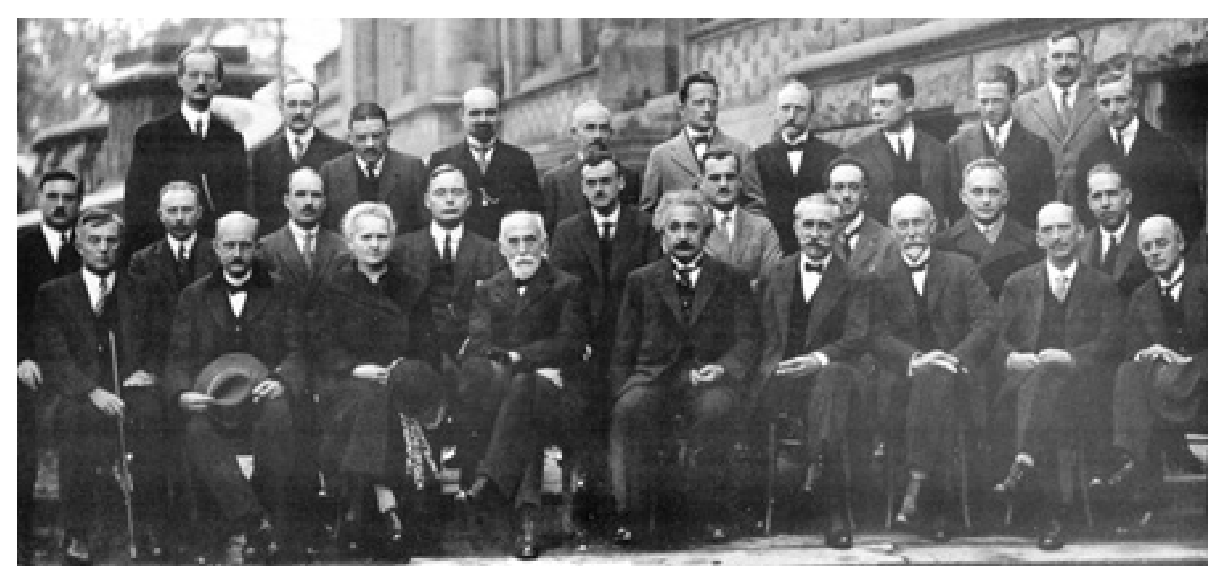
\includegraphics[clip,width=10cm]{1DProblem/1927solvay.ps}\\
\caption{1927年索尔维会议参加者,
这里有很多创立量子力学的物理学家。}\label{1927solvay}
\end{center}
\end{figure}


\subsection{一维定态的一般性质}

设微观粒子质量$m$,沿$x$轴运动,势能为$V(x)$,薛定鄂方程为:

\begin{center}
\begin{equation}
    i\hbar \frac{\partial }{{\partial t}}\psi (x,t) = \left[ { - \frac{{\hbar ^2 }}{{2m}}\frac{{\partial ^2 }}{{\partial x^2 }} + V(x)} \right]\psi (x,t)
\end{equation}
\end{center}

定态,系统具有确定能量E,波函数可以表示为:$\psi (x,t) = \psi (x)\exp \left( { - {\textstyle{{iEt} \over \hbar }}} \right)$

波函数$\psi (x)$满足:

\begin{center}
\begin{equation}
    \left[ { - \frac{{\hbar ^2 }}{{2m}}\frac{{d^2 }}{{dx^2 }} + V(x)} \right]\psi (x) = E\psi (x)
\end{equation}
\end{center}

或写为:$\psi '' + \frac{{2m}}{{\hbar ^2 }}\left[ {E - V(x)} \right]\psi  = 0$,是二阶齐次线性微分方程。

在量子力学中,势能V(x)取实数:$V^* (x) = V(x)$

\textbf{性质1:}如$\psi (x)$是一维定态薛定鄂方程的解,对应能量本征值为E,则$\psi ^* (x)$也是一维定态薛定鄂方程的解,对应能量也为E。

证明:$\left[ { - \frac{{\hbar ^2 }}{{2m}}\frac{{d^2 }}{{dx^2 }} + V(x)} \right]\psi (x) = E\psi (x)$,方程左右两边取复共轭,利用:$V^* (x) = V(x)$

$\left[ { - \frac{{\hbar ^2 }}{{2m}}\frac{{d^2 }}{{dx^2 }} + V(x)} \right]\psi ^* (x) = E^* \psi ^* (x) = E\psi ^* (x)$,$E^*  = E$\footnote{物理上允许的能量取值应为实数。}

\textbf{性质2:}如能级E非简并,对应能量本征函数总可取为实函数。

证明:能级非简并,$\psi (x)$,$\psi ^* (x)$描述同一个量子态,最多可相差一个常数因子:

\begin{center}
$\psi (x) = C\psi ^* (x) = C\left( {C\psi ^* (x)} \right)^*  = CC^* \psi (x) = \left| C \right|^2 \psi (x)$
\end{center}

$\left| C \right|^2  = 1,C = e^{i\alpha } ,\alpha  \in real$,可以取$\alpha  = 0$,$C = 1,\psi (x) = \psi ^* (x)$

即$\psi (x)$可取实函数。

\textbf{性质3:}如势函数V(x)具有空间反演对称,V(-x)=V(x),如$\psi (x)$是一维定态薛定谔方程的一个解,能量本征值为E,则$\psi ( - x)$也是方程的解,对应能量本征值也是E。

证明:$x \to  - x$,$\frac{{d^2 }}{{d( - x)^2 }} = \frac{{d^2 }}{{dx^2 }},V( - x) = V(x)$

$ - \frac{{\hbar ^2 }}{{2m}}\frac{{d^2 }}{{d( - x)^2 }}\psi ( - x) + V( - x)\psi ( - x) = E\psi ( - x) \to $

$ - \frac{{\hbar ^2 }}{{2m}}\frac{{d^2 }}{{dx^2 }}\psi ( - x) + V(x)\psi ( - x) = E\psi ( - x)$,得证

\textbf{性质4:}如势函数V(x)具有空间反演对称,V(-x)=V(x),
则对任意一个能量本征值E,存在一组完备解,其中每个波函数都有确定的宇称(奇偶性)。

证明:如$\psi (x)$是解,则$\psi ( - x)$也是解,对应能量本征值都是E。可以用$\psi (x)$,$\psi ( - x)$构造具有确定宇称的波函数:

\begin{center}
$\begin{array}{l}
 f(x) = \psi (x) + \psi ( - x) = f( - x) \\
 g(x) = \psi (x) - \psi ( - x) =  - g( - x) \\
 \end{array}$
\end{center}

$f(x)$,$g(x)$也是方程的解,对应能量本征值为E。

\subsection{可严格求解的单体定态问题}

真正可以严格求解的量子力学问题是很少的。对非相对论性量子力学而言,常见的可以严格求解的单粒子量子力学问题包括:

\begin{itemize}
  \item 无限深势阱
  \item 有限深势阱
  \item $\delta$势(Delta potential)
  \item 简谐振子
  \item 双曲正割平方势(Hyperbolic Secant-squared Potential)和余切平方势(Squared Cotangent
  Potential)\footnote{参考: 钱伯初, 曾谨言, 《量子力学习题精选与剖析》, 第1.9题和第1.10题。}
  \item 氢原子问题(当然,这是个典型的三维定态问题)
\end{itemize}

其中最简单的当然又属无限深势阱(The Infinite Square
Well)问题,该模型虽然简单,但仍可用来描述一些有趣的物理系统,比如导电聚合物(polymers)中的$\pi$电子\footnote{参考:M
V Volkenstein, Physics and Biology, pp15}。



\subsection{练习:无限深势阱}


\index{Infinite square well: 无限深势阱}

质量为$m$的粒子在一维无限深势阱(1D Infinite Square Well)中运动:

\begin{center}
$V(x) = \left\{ \begin{array}{l}
 0,x \in \left( {0,a} \right) \\
 \infty ,x \notin \left( {0,a} \right) \\
 \end{array} \right.$
\end{center}
\begin{itemize}
    \item 列出粒子的薛定谔方程;

    \item 求出归一化波函数;求出粒子在空间中的几率分布$w(x) = \psi ^* (x)\psi (x)dx$,并与``经典粒子''在空间中的出现几率进行比较;证明波函数的正交归一性:$\left\langle {n}
 \mathrel{\left | {\vphantom {n m}}
 \right. \kern-\nulldelimiterspace}
 {m} \right\rangle  = \delta _{m,n} $

    \item 求出粒子能量表达式;基态能量是多少?与经典粒子能量$E_k  = \frac{{p^2 }}{{2m}}$进行比较,说明在大量子数($n \to \infty $)时,粒子能量与经典粒子能量相符。

    \item 假设粒子在不同能级间跃迁,能量以光子形式放出$h\nu  = E_2  - E_1 $,求光谱的红限(频率最小光子对应的波长)是多少?

    \item $\psi  = \psi _n $时,$\left\langle x \right\rangle  = ?,\left\langle {p_x } \right\rangle  = ?$

\end{itemize}

若粒子束缚在边长为$a$,$b$,$c$的三维盒子中运动:

\begin{center}
$V(x,y,z) = \left\{ \begin{array}{l}
 0,x \in \left( {0,a} \right),y \in \left( {0,b} \right),z \in (0,c) \\
 \infty ,others \\
 \end{array} \right.$
\end{center}

\begin{itemize}
    \item 列出粒子的薛定谔方程,利用分离变量法($\psi (x,y,z) = \psi (x)\psi (y)\psi (z)$)求解薛定谔方程;
    \item 求出归一化波函数;并验证波函数的正交性:
    
\begin{equation*}
\left\langle {{n,m,l}}
 \mathrel{\left | {\vphantom {{n,m,l} {n',m',l'}}}
 \right. \kern-\nulldelimiterspace}
 {{n',m',l'}} \right\rangle  = \delta _{nn'} \delta _{mm'} \delta _{ll'} 
\end{equation*}
    
    
   \item 求出粒子能量表达式;
   
    \item 假设$a=b=c$,粒子基态能量是多少,写出归一化的基态波函数;粒子第一激发态能量是多少,并写出对应归一化波函数;(第一激发态能级是三重简并的,即相同能量本征值对应三个不同波函数或量子态)
    \item 求出第二激发态,第三激发态,第四激发态能级能量,并分别说明它们的能级是几重简并的。
    \item 费米子(Fermion)按泡利不相容原理,不能占据相同的量子态,假设有2个无自旋费米子(即不考虑自旋简并,每个量子态只能由一个费米子占据),不考虑无自旋费米子之间相互作用,求系统基态能是多少?
    \item 玻色子(Boson)不服从泡利不相容原理,可以占据相同量子态,在低温下,玻色子趋于占据最低能级,假设有2个玻色子,不考虑他们之间的相互作用,求系统基态能是多少?

   \end{itemize}

\index{Fermion: 费米子}

\index{Boson: 玻色子}

\textbf{解}:

(1)粒子薛定谔方程:$\left[ { - \frac{{\hbar ^2 }}{{2m}}\frac{{d^2 }}{{dx^2 }} + V(x)} \right]\psi (x) = E\psi (x)$


当$x \in \left( {0,a} \right)$时,$ - \frac{{\hbar ^2 }}{{2m}}\frac{{d^2 }}{{dx^2 }}\psi (x) = E\psi (x)$,即:

\begin{equation}\label{9-1-1}
\psi ''(x) + \frac{{2mE}}{{\hbar ^2 }}\psi (x) = 0
\end{equation}

当$x \notin \left( {0,a} \right),V(x) \to \infty $,即$x \notin \left( {0,a} \right),\psi (x) = 0$(否则,$\left\langle \psi  \right|V(x)\left| \psi  \right\rangle  \to \infty $,不是物理解)


针对$x \in \left( {0,a} \right)$区域,求解方程~\ref{9-1-1}


令$k^2  = \frac{{2mE}}{{\hbar ^2 }}$,则方程~\ref{9-1-1}化为:


\begin{equation}\label{9-1-2}
\psi '' + k^2 \psi  = 0
\end{equation}

$\psi (x) = Ae^{ikx}  + Be^{ - ikx} $是方程~\ref{9-1-2}的解,别代表向x轴正向和x轴负向传播的平面波。

边界条件:

$x=0$,$\psi (0) = A + B = 0$,即:$A=-B$


$x=a$,$\psi (a) = Ae^{ika}  + Be^{ - ika}  = A(e^{ika}  - e^{ - ika} ) = 2iA\sin ka = 0$,即:$\sin ka = 0$


即:$ka = n\pi ,n = 1,2...$,$k = \frac{{n\pi }}{a}$


所以波函数为:$\psi (x) = A\left( {e^{ikx}  - e^{ - ikx} } \right) = 2iA\sin kx = C\sin kx$,$k = \frac{{n\pi }}{a}$


(2)波函数归一化:

$\int_0^a {\left| C \right|^2 \sin ^2 \left( {\frac{{n\pi x}}{a}} \right)} dx = \int_0^a {\frac{{\left| C \right|^2 }}{2}\left( {1 - \cos \frac{{2n\pi x}}{a}} \right)} dx = \frac{{\left| C \right|^2 a}}{2} = 1$

所以:$\left| C \right| = \sqrt {\frac{2}{a}} $


归一化波函数可写为:$\psi (x) = \sqrt {{\textstyle{2 \over a}}} \sin {\textstyle{{n\pi x} \over a}},n = 1,2,...$


正交性:

\begin{eqnarray*}
\left\langle {n}
 \mathrel{\left | {\vphantom {n m}}
 \right. \kern-\nulldelimiterspace}
 {m} \right\rangle & = & \int_0^a {{\textstyle{2 \over a}}\sin {\textstyle{{n\pi x} \over a}}\sin {\textstyle{{m\pi x} \over a}}dx} \\
{} & = & \int_0^a {{\textstyle{2 \over a}}} \left( { - {\textstyle{1 \over 2}}} \right)\left( {\cos {\textstyle{{(n + m)\pi x} \over a}} - \cos {\textstyle{{(n - m)\pi x} \over a}}} \right)dx 
\end{eqnarray*}

利用三角和差与积公式:

\begin{equation}
\sin \alpha \sin \beta  =  - \frac{1}{2}\left( {\cos \left( {\alpha  + \beta } \right) - \cos \left( {\alpha  - \beta } \right)} \right)
\end{equation}


当$n \ne m$时,$\left\langle {n}
 \mathrel{\left | {\vphantom {n m}}
 \right. \kern-\nulldelimiterspace}
 {m} \right\rangle  = 0$;$n=m$时,$\left\langle {n}
 \mathrel{\left | {\vphantom {n m}}
 \right. \kern-\nulldelimiterspace}
 {m} \right\rangle  = \int_0^a {{\textstyle{1 \over a}}} dx = 1$


空间分布几率:$w(x) dx = \psi ^* \psi dx = {\textstyle{2 \over a}}\sin ^2 {\textstyle{{n\pi x} \over a}}dx$

经典粒子空间分布几率:$w(x) = \frac{{dt}}{T} = \frac{{{\raise0.5ex\hbox{$\scriptstyle {dx}$}
\kern-0.1em/\kern-0.15em
\lower0.25ex\hbox{$\scriptstyle v$}}}}{T} = \frac{{{\raise0.5ex\hbox{$\scriptstyle {dx}$}
\kern-0.1em/\kern-0.15em
\lower0.25ex\hbox{$\scriptstyle v$}}}}{{{\raise0.5ex\hbox{$\scriptstyle a$}
\kern-0.1em/\kern-0.15em
\lower0.25ex\hbox{$\scriptstyle v$}}}} = \frac{1}{a}dx$

即:经典粒子出现几率是``平均分布''的,而量子情形则与粒子具体位置有关。


(3)能级:$E_n  = \frac{{\hbar ^2 k^2 }}{{2m}} = \frac{{\hbar ^2 }}{{2m}}\left( {\frac{{n\pi }}{a}} \right)^2  = \frac{{n^2 \pi ^2 \hbar ^2 }}{{2ma^2 }},n = 1,2,...$


基态能量对应最低能量,$E_1  = \frac{{\pi ^2 \hbar ^2 }}{{2ma^2 }}$


经典动能:$E_k  = \frac{{p^2 }}{{2m}}$,连续取值,从0到无穷大,而量子情形只能取分立值(量子化)。



大量子数时,$\Delta E(n) = \frac{{\pi ^2 \hbar ^2 }}{{2ma^2 }}\left[ {\left( {n + 1} \right)^2  - n^2 } \right] = \frac{{\pi ^2 \hbar ^2 }}{{2ma^2 }}\left( {2n + 1} \right)$


$n \to \infty $,$\frac{{\Delta E(n)}}{{E_n }} = \frac{{2n + 1}}{{n^2 }} \sim \frac{2}{n} \to 0$,

即在大量子数时,能级间距与能级本身比较是可以忽略不计的,即具有``准连续''性。另外:$E_n  = \frac{{n^2 \pi ^2 \hbar ^2 }}{{2ma^2 }} = \frac{{\left( {\hbar k} \right)^2 }}{{2m}}$,具有和经典粒子一样的形式,只是取值是分立的。所以:在大量子数($n \to \infty $)时,粒子能量与经典粒子能量相符。


(4)相邻能级能量差:

\begin{equation}
\Delta E(n) = \frac{{\pi ^2 \hbar ^2 }}{{2ma^2 }}\left[ {\left( {n + 1} \right)^2  - n^2 } \right] = \frac{{\pi ^2 \hbar ^2 }}{{2ma^2 }}\left( {2n + 1} \right)
\end{equation}

$n=1$时,能级差最小:$h\nu  = h\frac{c}{\lambda } = \frac{{3\pi ^2 \hbar ^2 }}{{2ma^2 }}$

所以:$\lambda _{\max }  = \frac{{2ma^2 hc}}{{3\pi ^2 \hbar ^2 }}$


(5)平均位置、平均动量:

$\left\langle x \right\rangle  = \left\langle n \right|x\left| n \right\rangle  = \int_0^a {{\textstyle{2 \over a}}} x\sin ^2 {\textstyle{{n\pi x} \over a}}dx = \int_0^a {\frac{x}{a}} \left( {1 - \cos {\textstyle{{2n\pi x} \over a}}} \right)dx = \frac{1}{a}\frac{{a^2 }}{2} = \frac{a}{2}$


$\left\langle {p_x } \right\rangle  = \left\langle n \right|\hat p_x \left| n \right\rangle  = \int_0^a {{\textstyle{2 \over a}}} \sin {\textstyle{{n\pi x} \over a}}\left( {\frac{\hbar }{i}\frac{d}{{dx}}} \right)\sin {\textstyle{{n\pi x} \over a}}dx = 0$


动量平均值为0,$\sin kx = \frac{{e^{ikx}  - e^{ - ikx} }}{{2i}}$可看作振幅相同传播方向相反平面波(或动量$\hbar k$自由粒子),所以平均为0。


(6)三维薛定谔方程:

\begin{equation}\label{9-1-3}
\left[ { - \frac{{\hbar ^2 }}{{2m}}\nabla ^2  + V(x,y,z)} \right]\psi (x,y,z) = E\psi (x,y,z)
\end{equation}


取直角坐标系,$\nabla ^2  = \frac{{\partial ^2 }}{{\partial x^2 }} + \frac{{\partial ^2 }}{{\partial y^2 }} + \frac{{\partial ^2 }}{{\partial z^2 }}$


当$x \in \left( {0,a} \right),y \in (0,b),z \in (0,c)$,方程~\ref{9-1-3}化为:


\begin{equation}\label{9-1-4}
\left[ { - \frac{{\hbar ^2 }}{{2m}}\left( {\frac{{\partial ^2 }}{{\partial x^2 }} + \frac{{\partial ^2 }}{{\partial y^2 }} + \frac{{\partial ^2 }}{{\partial z^2 }}} \right)} \right]\psi (x)\psi (y)\psi (z) = E\psi (x)\psi (y)\psi (z)
\end{equation}


定义:$k^2  = \frac{{2mE}}{{\hbar ^2 }}$,


方程~\ref{9-1-4}化为:$\psi ''_x \psi _y \psi _z  + \psi _x \psi ''_y \psi _z  + \psi _x \psi _y \psi ''_z  + k^2 \psi _x \psi _y \psi _z  = 0$


两边同时除$\psi _x \psi _y \psi _z $

$\frac{{\psi ''_x }}{{\psi _x }} + \frac{{\psi ''_y }}{{\psi _y }} + \frac{{\psi ''_z }}{{\psi _z }} + k^2  = 0$


即:$\frac{{\psi ''(x)}}{{\psi (x)}} + k_x ^2  = 0,\frac{{\psi ''(y)}}{{\psi (y)}} + k_y ^2  = 0,\frac{{\psi ''(z)}}{{\psi (z)}} + k_z ^2  = 0$,$k^2  = k_x ^2  + k_y ^2  + k_z ^2 $


解的形式与一维类似:

$\begin{array}{l}
 \psi (x) = \sqrt {{\textstyle{2 \over a}}} \sin {\textstyle{{n\pi x} \over a}},n = 1,2,... \\
 \psi (y) = \sqrt {{\textstyle{2 \over b}}} \sin {\textstyle{{m\pi y} \over b}},m = 1,2,... \\
 \psi (z) = \sqrt {{\textstyle{2 \over c}}} \sin {\textstyle{{l\pi z} \over c}},l = 1,2,... \\
 \end{array}$

(7)归一化波函数:

$\psi (x,y,z) = \sqrt {{\textstyle{8 \over {abc}}}} \sin {\textstyle{{n\pi x} \over a}}\sin {\textstyle{{m\pi y} \over b}}\sin {\textstyle{{l\pi z} \over c}}$

正交关系:

\begin{eqnarray*}
{} & {} & \left\langle {{n,l,m}}
 \mathrel{\left | {\vphantom {{n,l,m} {n',l',m'}}}
 \right. \kern-\nulldelimiterspace}
 {{n',l',m'}} \right\rangle  =  \\
{} & {} &  \frac{8}{{abc}}\int_0^a {\sin {\textstyle{{n\pi x} \over a}}\sin {\textstyle{{n'\pi x} \over a}}dx\int_0^b {\sin {\textstyle{{m\pi y} \over a}}\sin {\textstyle{{m'\pi y} \over a}}dy} } \int_0^c {\sin {\textstyle{{l\pi z} \over a}}\sin {\textstyle{{l'\pi z} \over a}}dz} 
\end{eqnarray*}

每个积分都与1D情形一样,所以:

\begin{equation*}
\left\langle {{n,m,l}}
 \mathrel{\left | {\vphantom {{n,m,l} {n',m',l'}}}
 \right. \kern-\nulldelimiterspace}
 {{n',m',l'}} \right\rangle  = \delta _{nn'} \delta _{mm'} \delta _{ll'} 
 \end{equation*}

(8)能级:

$k^2  = k_x ^2  + k_y ^2  + k_z ^2  = \left( {{\textstyle{{n\pi } \over a}}} \right)^2  + \left( {{\textstyle{{m\pi } \over b}}} \right)^2  + \left( {{\textstyle{{l\pi } \over c}}} \right)^2 $

所以:$E_{n,l,m}  = \frac{{\hbar ^2 }}{{2m}}\left[ {\left( {\frac{{n\pi }}{a}} \right)^2  + \left( {\frac{{m\pi }}{b}} \right)^2  + \left( {\frac{{l\pi }}{c}} \right)^2 } \right]$

(9)$a=b=c$,

基态能量:$E_{111}  = \frac{{3\hbar ^2 \pi ^2 }}{{2ma^2 }}$

$\psi _{111}  = \sqrt {{\textstyle{8 \over {a^3 }}}} \sin {\textstyle{{\pi x} \over a}}\sin {\textstyle{{\pi y} \over a}}\sin {\textstyle{{\pi z} \over a}}$


第一激发态:$E_{211}  = E_{121}  = E_{112}  = \frac{{6\hbar ^2 \pi ^2 }}{{2ma^2 }} = \frac{{3\hbar ^2 \pi ^2 }}{{ma^2 }}$

对应波函数有三个:

$\begin{array}{l}
 \psi _{211}  = \sqrt {{\textstyle{8 \over {a^3 }}}} \sin {\textstyle{{2\pi x} \over a}}\sin {\textstyle{{\pi y} \over a}}\sin {\textstyle{{\pi z} \over a}} \\
 \psi _{121}  = \sqrt {{\textstyle{8 \over {a^3 }}}} \sin {\textstyle{{\pi x} \over a}}\sin {\textstyle{{2\pi y} \over a}}\sin {\textstyle{{\pi z} \over a}} \\
 \psi _{112}  = \sqrt {{\textstyle{8 \over {a^3 }}}} \sin {\textstyle{{\pi x} \over a}}\sin {\textstyle{{\pi y} \over a}}\sin {\textstyle{{2\pi z} \over a}} \\
 \end{array}$

(10)

第二激发态:$E_{221}  = E_{122}  = E_{212}  = \frac{{9\hbar ^2 \pi ^2 }}{{2ma^2 }}$, (简并度=3)
\footnote{如果一个能级对应一个波函数,则称能级是非简并的;如果一个能级对应多个不同的波函数,
则称能级是简并的,有几个不同波函数对应于同一个能级,则该能级的简并度就是几。}

第三激发态:$E_{311}  = E_{131}  = E_{113}  = \frac{{11\hbar ^2 \pi ^2 }}{{2ma^2 }}$, (简并度=3)

第四激发态:$E_{222}  = \frac{{12\hbar ^2 \pi ^2 }}{{2ma^2 }} = \frac{{6\hbar ^2 \pi ^2 }}{{ma^2 }}$. (非简并)

(11)2个无自旋费米子组成系统的基态能:

$E = E_{111}  + E_{211}  = E_{111}  + E_{121}  = E_{111}  + E_{112}  = \frac{{9\hbar ^2 \pi ^2 }}{{2ma^2 }}$


(12)2个玻色子组成系统的基态能:

$E = 2E_{111}  = \frac{{3\hbar ^2 \pi ^2 }}{{ma^2 }}$


\subsection*{阅读与思考}



有限深方势阱, 深度为$V_0$, 定性证明:当$E \in \left[ { - V_0 ,0}
\right]$时, 只存在分立能级, 即假设$E_0$是本征值,
$E_0$邻域内只存在$E_0$一个解。

当$E > 0$时, 只存在连续能级, 即假设$E_0$是本征值,
$E_0$邻域内存在除$E_0$之外的解。
